\documentclass[letterpaper,12pt]{article}

% --- PAQUETES DE IDIOMA ---
\usepackage[spanish,mexico]{babel}
\usepackage[utf8]{inputenc}
\usepackage{csquotes}
\usepackage[T1]{fontenc}

% --- PAQUETES MATEMÁTICOS ---
\usepackage{amsmath}
\usepackage{amssymb}
\usepackage{cancel}
\usepackage{mathrsfs}

% --- PAQUETES GRÁFICOS Y DE DISEÑO ---
\usepackage{graphicx}
\usepackage{float}
\usepackage{subcaption}
\usepackage[table]{xcolor}
\usepackage{longtable}
\usepackage{multirow}
\usepackage{makecell}
\usepackage{array}
\usepackage{caption}
\usepackage{tikz}
\usetikzlibrary{decorations.pathreplacing}
\usetikzlibrary{decorations.pathmorphing}
\usetikzlibrary{positioning}

% --- DIBUJAR CIRCUITOS ---
\usepackage{circuitikz}
\usetikzlibrary{shapes.geometric, shapes.multipart, shapes.symbols, positioning, arrows.meta, calc, shadows, decorations.pathreplacing,babel}


% --- MAPAS DE KARNAUGH ---
\usepackage{karnaugh-map}

% --- LISTAS ---
\usepackage{enumitem}

% --- PAQUETES DE CÓDIGO ---
\usepackage{listings}
% Configuración de colores para listings
\definecolor{codebg}{rgb}{0.95,0.95,0.95}
\definecolor{keyword}{rgb}{0.0,0.2,0.6}
\definecolor{comment}{rgb}{0.25,0.5,0.35}
\definecolor{string}{rgb}{0.6,0.0,0.0}
\definecolor{number}{rgb}{0.5,0.0,0.5}
\definecolor{codegray}{rgb}{0.5,0.5,0.5}
\definecolor{codepurple}{rgb}{0.58,0,0.82}
\definecolor{backcolour}{rgb}{0.95,0.95,0.95}

% Configuración general 
\lstset{
    backgroundcolor=\color{backcolour},
    inputencoding=utf8,
    keywordstyle=\color{blue}\bfseries,
    stringstyle=\color{codepurple},
    commentstyle=\color{codegray}\itshape,
    numbers=left,
    numberstyle=\tiny\color{codegray},
    frame=single,
    rulecolor=\color{black},
    breaklines=true,
    tabsize=4,
    showstringspaces=false,
    extendedchars=true,
    literate={á}{{\'a}}1
             {é}{{\'e}}1
             {í}{{\'i}}1
             {ó}{{\'o}}1
             {ú}{{\'u}}1
             {Á}{{\'A}}1
             {É}{{\'E}}1
             {Í}{{\'I}}1
             {Ó}{{\'O}}1
             {Ú}{{\'U}}1
             {ñ}{{\~n}}1
             {Ñ}{{\~N}}1
             {¿}{{\textquestiondown}}1
             {¡}{{\textexclamdown}}1
             {°}{{\textdegree}}1
             {ø}{{\o}}1
}

% --- CONFIGURACIÓN ESPECÍFICA PARA VHDL ---
\lstdefinestyle{estiloVHDL}{
    language=VHDL,
    basicstyle=\ttfamily\footnotesize,
    backgroundcolor=\color{codebg},
    commentstyle=\color{comment}\itshape,
    keywordstyle=\color{keyword}\bfseries,
    numberstyle=\tiny\color{codegray},
    stringstyle=\color{string},
    breakatwhitespace=false,         
    breaklines=true,                 
    captionpos=b,                    
    keepspaces=true,                 
    numbers=left,                    
    numbersep=5pt,                  
    showspaces=false,                
    showstringspaces=false,
    showtabs=false,                  
    tabsize=4,
    frame=single,
    rulecolor=\color{black},
    % Librerías y tipos comunes de VHDL para el resaltado
    morekeywords={
        library,use,all,entity,is,port,in,out,inout,buffer,architecture,of,
        begin,end,signal,variable,constant,type,array,downto,to,if,then,else,
        elsif,case,when,with,select,generate,for,while,process,wait,map,
        generic,component,std_logic,std_logic_vector,ieee,std_logic_1164,
        numeric_std,unsigned,signed,integer,boolean
    }
}

% --- RUTAS DE IMÁGENES ---
\graphicspath{{img/}{portada_img/}}

% --- CONFIGURACIÓN DE PÁGINA ---
\usepackage[
    left=25mm, 
    right=25mm,
    top=35mm,
    bottom=30mm,
    headheight=15pt, 
    papersize={21.59cm,27.94cm}
]{geometry}

% --- FORMATO DE TEXTO ---
\renewcommand{\baselinestretch}{1.25} 
\usepackage{parskip} 
\usepackage{lipsum}

% --- VARIABLES GLOBALES ---
\newcommand{\materia}{Laboratorio de Organización y Arquitectura de Computadoras}

% --- ENCABEZADOS Y PIES DE PÁGINA ---
\usepackage{fancyhdr}
\pagestyle{fancy}
\fancyhf{} 

% --- CONFIGURACIÓN DE ENCABEZADO Y PIE DE PÁGINA ---
\fancyhead[L]{} 
%
\fancyhead[R]{\textsc{\materia}}   

\fancyfoot[C]{\thepage} 
% Linea Encabezado y Pie de Página
\renewcommand{\headrulewidth}{0.8pt} 
\renewcommand{\footrulewidth}{0pt}

% --- BIBLIOGRAFÍA ---
\usepackage[backend=biber, style=numeric, sorting=none, url=true]{biblatex}
% \addbibresource{referencias.bib}

% --- HIPERVÍNCULOS ---
\usepackage{hyperref}
\hypersetup{
    colorlinks=true,
    linkcolor=blue,
    citecolor=blue,
    filecolor=magenta,
    urlcolor=cyan
}

\renewcommand{\baselinestretch}{1.0}


\begin{document}
    % --- PORTADA ---
    \thispagestyle{empty} % Sin encabezado ni pie en la portada

% --- ENCABEZADO DE PORTADA (TABLA DE 3 COLUMNAS) ---
\begin{center}
    % La tabla usa 'm' para centrar verticalmente las imágenes y el texto
    \begin{tabular}{m{0.15\textwidth} m{0.60\textwidth} m{0.15\textwidth}}
        % Logo Izquierdo (UNAM)
        
\includegraphics[width=2cm]{portada_img/escudounam_negro.jpg} & 
        
        % Título Central
        \centering\Huge\textbf{Universidad Nacional Autónoma de México} &
        
        % Logo Derecho (Facultad)
        \raggedleft
\includegraphics[width=2cm]{portada_img/escudofi_negro.jpg}
    \end{tabular}
\end{center}

\vspace{0.3cm}

% --- INFORMACIÓN DEL REPORTE ---
\begin{center}
    {\LARGE \textbf{Facultad de Ingeniería}}\\[1cm]

    {\LARGE \textbf{Laboratorio de Arquitectura y Organización de Computadoras}} \\[1cm]

	{\LARGE Grupo: 07 - Semestre: 2027-1} \\[1cm]
    
    {\LARGE \textbf{Reporte Practica 2 Pt.1}}\\[0.5cm]
    {\LARGE {Diseño de máquinas de estado}}\\[1cm]

    {\Large \textbf{Fecha de Entrega}}\\[0.2cm]
    {\Large 04 de Septiembre del 2026} \\[1cm]

    {\LARGE \textbf{Profesor}}\\[0.2cm]
    {\Large Ing. Julio Cesar Cruz Estrada}\\[1cm]
    
    {\LARGE \textbf{Integrantes:}}\\[0.2cm]
    {\Large Espinoza Matamoros Percival Ulises}\\[0.5cm]
    {\Large Montiel Juárez Oscar Iván}\\[0.5cm]
    {\Large Veraza García Amy Valentina}\\[0.5cm]

\end{center} 
    \newpage
    
    
    % --- Indice ---
    % \tableofcontents
    % \newpage

    % --- CONTENIDO DEL DOCUMENTO ---
    \section{Objetivo}
    Familiarizar al alumno en el conocimiento de los algoritmos de las máquinas de estados utilizando Quartus y el lenguaje VHDL.


    \section{Desarrollo}

    A partir dela carta ASM que se proporciona en la práctica (Figura [\ref{fig:carta_asm}]) se solicita obtener su circuito secuencial utilizando flip-flops tipo D. Ademas se debe de implementar el circuito en el ambiente de desarrollo Quartus.

    \begin{figure}[H]
        \centering
        \begin{tikzpicture}[
            scale=1.0, transform shape,
            % Estilos de los nodos
            state/.style={rectangle, draw, minimum width=3cm, minimum height=1.5cm, align=center},
            decision/.style={diamond, draw, aspect=1.5, minimum width=2.5cm, minimum height=2.5cm, align=center},
            arrow/.style={->, >=Stealth, semithick}
        ]

            % Definición de nodos
            \node[state, label=left:Edo0] (edo0) {};
            \node[decision, below=0.8cm of edo0] (go) {GO};
            \node[state, label=left:Edo1, below=0.8cm of go] (edo1) {RESET};
            \node[decision, below=0.8cm of edo1] (fc) {FC};
            \node[state, label=left:Edo2, below=0.8cm of fc] (edo2) {DONE};

            % Conexiones del flujo principal y valores '1'
            \draw[arrow] (edo0) -- (go);
            \draw[arrow] (go.south) -- node[left] {1} (edo1.north);
            \draw[arrow] (edo1) -- (fc);
            \draw[arrow] (fc.south) -- node[left] {1} (edo2.north);

            % Retornos con valor '0' (por la derecha)
            \draw[arrow] (go.east) -- node[above, near start] {0} ++(2,0) |- ($(edo0.north) + (0,0.5)$) -- (edo0.north);
            \draw[arrow] (fc.east) -- node[above, near start] {0} ++(2,0) |- ($(edo1.north) + (0,0.5)$) -- (edo1.north);

            % Retorno final desde Edo2 a Edo0 (por la izquierda)
            \draw[arrow] (edo2.south) -- ++(0,-0.6) -| ($(edo0.west) + (-2,0)$) |- ($(edo0.north) + (0,0.5)$);
        \end{tikzpicture}
        \caption{Carta ASM Práctica 2}
        \label{fig:carta_asm}
    \end{figure}

    Para obtener el circuito secuencial a partir de la carta ASM, se debe de realizar la tabla de transición de estados y la tabla de salida:

    \begin{table}[h]
        \centering
        \begin{tabular}{|c|c|c|c|c|c|c|c|c|}
        \hline
        \multirow{2}{*}{} & \multicolumn{2}{c|}{\textbf{Estado Presente}} & \multicolumn{2}{c|}{\textbf{Entradas}} & \multicolumn{2}{c|}{\textbf{Estado Siguiente}} & \multicolumn{2}{c|}{\textbf{Salidas}} \\ \cline{2-9} 
        & $Q_1$ & $Q_0$ & $GO$ & $FC$ & ${Q_1}^+$ & ${Q_0}^+$ & $RESET$ & $DONE$ \\ \hline
        \multirow{2}{*}{Edo0} & 0 & 0 & 0 & * & 0 & 0 & 0 & 0 \\ \cline{2-9} 
        & 0 & 0 & 1 & * & 0 & 1 & 0 & 0 \\ \hline
        \multirow{2}{*}{Edo1} & 0 & 1 & * & 0 & 0 & 1 & 1 & 0 \\ \cline{2-9} 
        & 0 & 1 & * & 1 & 1 & 0 & 1 & 0 \\ \hline
        Edo2 & 1 & 0 & * & * & 0 & 0 & 0 & 1 \\ \hline
        \end{tabular}
        \caption{Tabla de Transición de Estados}
        \label{tab:transicion}
    \end{table}

    Obteniendo las ecuaciones por medio de mapas de Karnaugh, se obtiene lo siguiente:

    \textbf{Reducción por medio de Mapas de Karnaugh: ${Q_0}^+$}
    \begin{center}
        \begin{karnaugh-map}[4][4][1][$Q_1 Q_0$][$GO \: FC$]
            \minterms{2,3,4,6}
             % Don't Care
            \terms{12,13,14,15}{$X$} 
            \autoterms[0]
            \implicant{3}{2}
            \implicantedge{4}{12}{6}{14}
        \end{karnaugh-map}
    \end{center}
    \vspace{-7mm}
    \[{{Q_0}^+} = Q_0 \: \overline{FC} + \overline{Q_1} \: Q_0 \: GO \]   

    \newpage
    \textbf{Reducción por medio de Mapas de Karnaugh: ${Q_1}^+$}
    \begin{center}
        \begin{karnaugh-map}[4][4][1][$Q_1 Q_0$][$GO \: FC$]
            \minterms{2,3,4,6}
             % Don't Care
            \terms{12,13,14,15}{$X$} 
            \autoterms[0]
            \implicant{5}{15}
        \end{karnaugh-map}
    \end{center}
    \vspace{-7mm}
    \[{{Q_1}^+} = Q_0 + FC \]  

    \textbf{Reducción por medio de Mapas de Karnaugh: $RESET$}
    \begin{center}
        \begin{karnaugh-map}[4][4][1][$Q_1 Q_0$][$GO \: FC$]
            \minterms{4,5,6,7}
             % Don't Care
            \terms{12,13,14,15}{$X$} 
            \autoterms[0]
            \implicant{4}{14}
        \end{karnaugh-map}
    \end{center}
    \vspace{-7mm}
    \[{RESET} = Q_0 \]  

    \textbf{Reducción por medio de Mapas de Karnaugh: $DONE$}
    \begin{center}
        \begin{karnaugh-map}[4][4][1][$Q_1 Q_0$][$GO \: FC$]
            \minterms{8,9,10,11}
             % Don't Care
            \terms{12,13,14,15}{$X$} 
            \autoterms[0]
            \implicant{12}{10}
        \end{karnaugh-map}
    \end{center}
    \vspace{-7mm}
    \[{DONE} = Q_1 \]  

    \section{Simulaciones}

    \lipsum[1-3]

    \section{Resultados}

    Para la verificación del funcionamiento del contador de 4 bits, se cargo el diseño digital a la tarjeta FPGA, para ello se seleccionó la opción \textit{Tools $\rightarrow$ Programmer}. Es importante mencionar que se debe de cargar el diseño que contiene el bloque del divisor de frecuencia, esto para poder visualizar el contador de 4 bits.

    \newpage

    \textbf{Contador de 4 bits cuando \texttt{reset = 0}}

    \begin{figure}[H]
        \centering
        % ---------- FILA SUPERIOR ----------
        \begin{subfigure}[b]{0.24\textwidth}
            \centering
            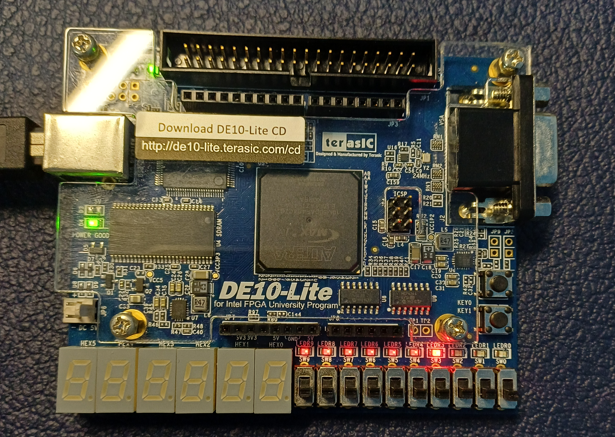
\includegraphics[width=\textwidth]{img/cont_1000.png}
            \caption{Contador de 4 bits (\texttt{1000})}
            \label{fig:img1}
        \end{subfigure}
        \hfill
        \begin{subfigure}[b]{0.24\textwidth}
            \centering
            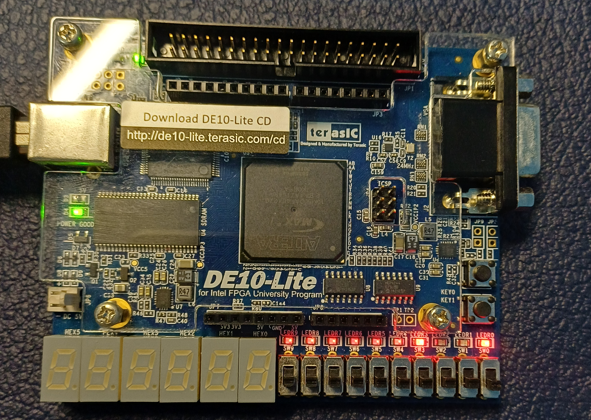
\includegraphics[width=\textwidth]{img/cont_1001.png}
            \caption{Contador de 4 bits (\texttt{1001})}
            \label{fig:img2}
        \end{subfigure}
        \hfill
        \begin{subfigure}[b]{0.24\textwidth}
            \centering
            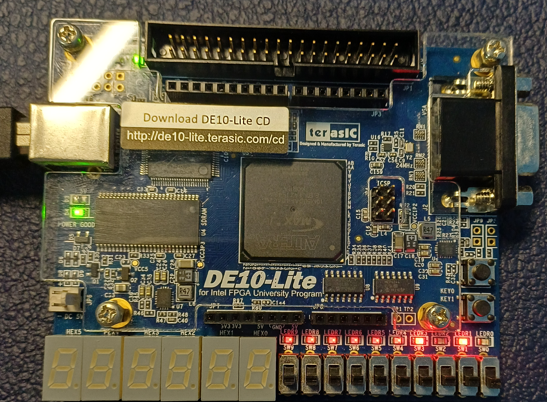
\includegraphics[width=\textwidth]{img/cont_1010.png}
            \caption{Contador de 4 bits (\texttt{1010})}
            \label{fig:img3}
        \end{subfigure}
        \hfill
        \begin{subfigure}[b]{0.24\textwidth}
            \centering
            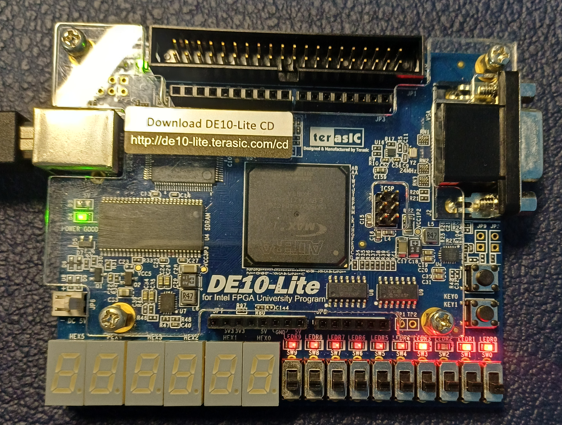
\includegraphics[width=\textwidth]{img/cont_1011.png}
            \caption{Contador de 4 bits (\texttt{1011})}
            \label{fig:img4}
        \end{subfigure}
        
        \vspace{0.5cm} 
        
        % ---------- FILA INFERIOR ----------
        \begin{subfigure}[b]{0.24\textwidth}
            \centering
            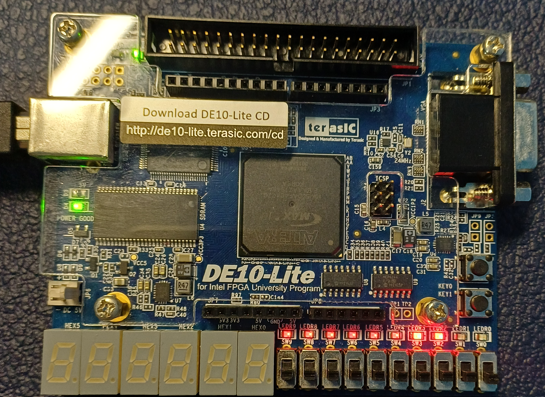
\includegraphics[width=\textwidth]{img/cont_1100.png}
            \caption{Contador de 4 bits (\texttt{1100})}
            \label{fig:img5}
        \end{subfigure}
        \hfill
        \begin{subfigure}[b]{0.24\textwidth}
            \centering
            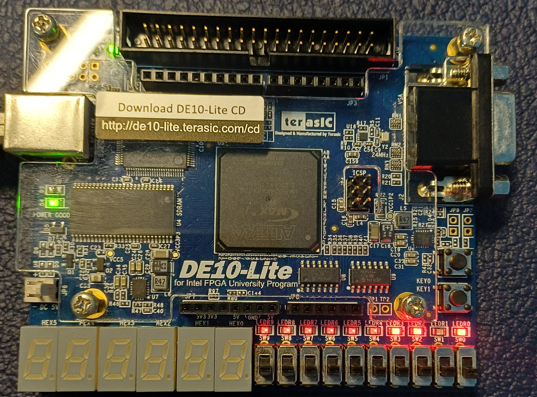
\includegraphics[width=\textwidth]{img/cont_1101.png}
            \caption{Contador de 4 bits (\texttt{1101})}
            \label{fig:img6}
        \end{subfigure}
        \hfill
        \begin{subfigure}[b]{0.24\textwidth}
            \centering
            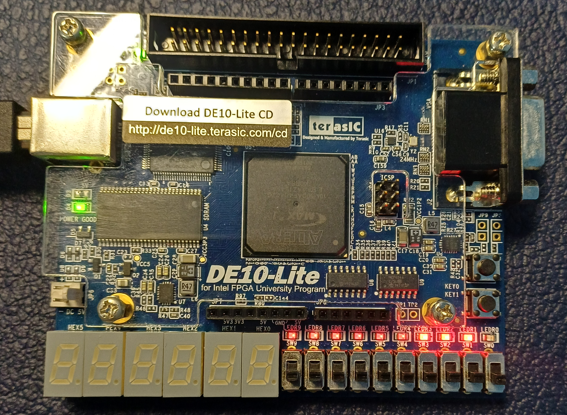
\includegraphics[width=\textwidth]{img/cont_1110.png}
            \caption{Contador de 4 bits (\texttt{1110})}
            \label{fig:img7}
        \end{subfigure}
        \hfill
        \begin{subfigure}[b]{0.24\textwidth}
            \centering
            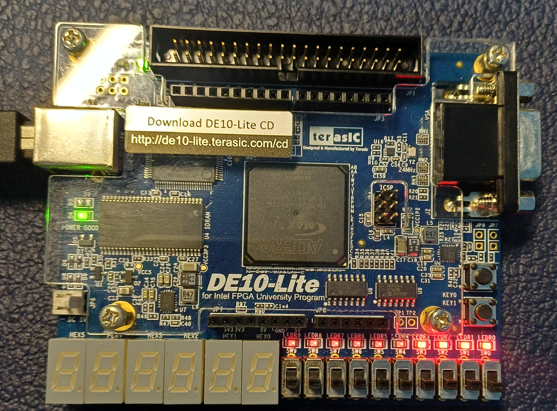
\includegraphics[width=\textwidth]{img/cont_1111.png}
            \caption{Contador de 4 bits (\texttt{1111})}
            \label{fig:img8}
        \end{subfigure}
        
        \caption{Algunos valores del Contador de 4 bits cuando reset = 0.}
        \label{fig:grid8}
    \end{figure}

    \textbf{Contador de 4 bits cuando \texttt{reset = 1}}

    \begin{figure}[H]
        \centering
        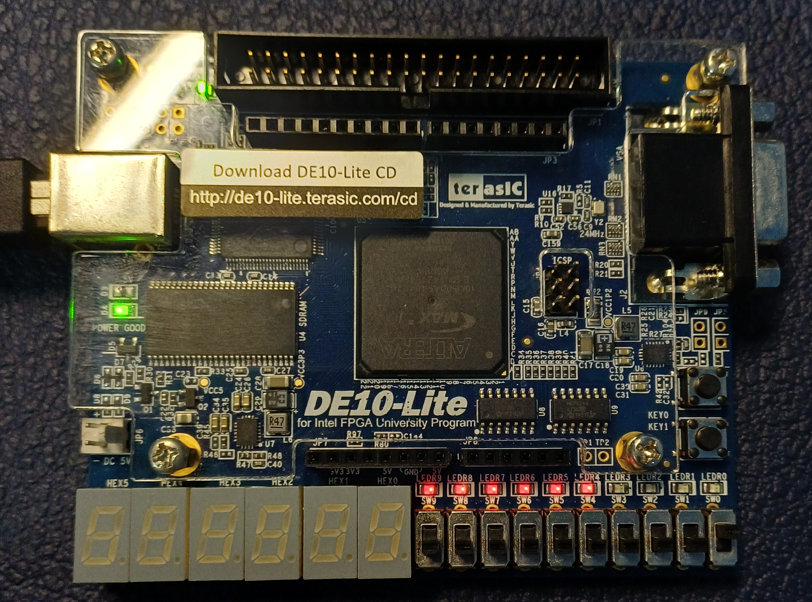
\includegraphics[width=0.55\linewidth]{img/cont_rst.png}
        \caption{Contador de 4 bits cuando \texttt{reset = 1}. (\texttt{0000})}
        \label{fig:cont_rst}
    \end{figure}

    \section{Conclusión}

    \textbf{Percival Ulises Espinoza Matamoros:} \lipsum[1]

    \textbf{Oscar Iván Montiel Juárez:} \lipsum[1]

    \textbf{Amy Valentina Veraza García:} \lipsum[1]

    % --- Referencias ---
    \nocite{*} 
    % \printbibliography[heading=bibintoc, title={Referencias}]
\end{document}
